\section{Hierarchical Bayesian estimates}\label{sec:bayes}

\subsection{Model}

The primary model keeps $\theta_i$ as the coefficient sum but lets countries borrow
strength from one another, and it models the dependence that the classical regressions
leave in the residuals. Write $y_{it}=\Delta u_{it}$ and reparameterise the lag weights so
that $\theta_i$ appears directly:
\begin{align}
  y_{it} &= \alpha_i + \theta_i\, g_{it} + \sum_{k=1}^{K} b_{ik}\,(g_{i,t-k}-g_{it})
            + \lambda_i f_t + e_{it}, \label{eq:bayes}\\
  e_{it} &= \phi_i\, e_{i,t-1} + \sigma_i\,\eta_{it},\qquad \eta_{it}\sim t_\nu ,
\end{align}
with $K=2$. Here:
\begin{itemize}
  \item $f_t\sim N(0,1)$ is a common quarterly factor with non-negative loadings
    $\lambda_i$, representing European shocks not captured by each country's own growth;
  \item the AR(1) term captures residual persistence;
  \item Student-$t$ innovations allow for outlying quarters.
\end{itemize}
Country parameters are partially pooled \citep{gelman2013bda} through non-centred
hierarchies, for example
$\theta_i=\mu_\theta+\tau_\theta z_i$ with $z_i\sim N(0,1)$. Analogous hierarchies apply
to $\alpha_i$, $b_{ik}$, $\phi_i$ (on the $\tanh$ scale) and $\log\sigma_i$.

\paragraph{Priors.} The prior on the mean sum, $\mu_\theta\sim N(0,0.5^2)$, is centred at
zero, so the prior does not assume Okun's law. The other priors are
$\tau_\theta\sim N^+(0,0.25^2)$, $\lambda_i\sim N^+(0,0.2^2)$ and
$\nu\sim\mathrm{Gamma}(2,0.1)$. Prior predictive checks show that these weakly informative
priors put visible mass on implausibly large quarterly changes. This is reported rather
than tuned.

\paragraph{Estimands.} $\mu_\theta$ is the mean of the population distribution of country
sums: an unweighted cross-country average. It is not an EU aggregate and not a pooled
slope. With the common factor in the model, $\theta_i$ measures the association with each
country's GDP growth beyond the common European cycle.

\paragraph{Sample.} The primary sample is 2009-Q2 to 2019-Q4: the longest window that is
contiguous and definition-consistent in every country.

\subsection{Posterior inference}

\paragraph{Sampler.} Posteriors are sampled with the No-U-Turn sampler
\citep{hoffman2014nuts} in NumPyro \citep{phan2019numpyro}: four chains of 1000 warm-up and
1000 retained draws, target acceptance $0.95$, fixed seeds.

\paragraph{Acceptance.} A fit is accepted only if all four conditions hold:
\begin{itemize}
  \item the rank-normalised $\widehat R\le 1.01$ \citep{vehtari2021rhat};
  \item bulk and tail effective sample sizes are at least 400;
  \item there are no divergences;
  \item E-BFMI $\ge 0.3$.
\end{itemize}
A failed fit is reported and not interpreted.

\paragraph{Sensitivity.} Nine specifications were fixed in advance: wide priors, strong
pooling, no pooling, no common factor, Gaussian i.i.d.\ errors, the participation control,
four lags, and a sample without 2020--2021. Of these, \val{by_n_accepted} of
\val{by_n_specs} were accepted; the unpooled fit missed the $\widehat R$ threshold.

\paragraph{Model comparison and checks.} Models are compared by PSIS-LOO
\citep{vehtari2017loo} and checked with posterior predictive statistics.

\subsection{Results}

\paragraph{Average and spread.} The mean country sum is $\mu_\theta=$ \val{by_mu} (90\%
credible interval \val{by_mu_ci}). The between-country standard deviation is
$\tau_\theta=$ \val{by_tau} (\val{by_tau_ci}).

\paragraph{Country signs.}
\begin{itemize}
  \item \val{by_n_neg_primary} of \val{n_countries} country sums are credibly negative,
    meaning $P(\theta_i<0)\ge 0.95$, in the primary fit;
  \item \val{by_n_neg_all} are credibly negative in every accepted specification.
\end{itemize}

\paragraph{Magnitudes.} The Bayesian sums are smaller in magnitude than OLS on the same
quarters in \val{by_n_smaller} of \val{n_countries} countries (table~\ref{tab:countries},
figure~\ref{fig:countries}). Pooling
explains only part of the difference. The error model and the common factor change the
estimand: the classical sum includes the common cycle, while the factor model's sum does
not.

\paragraph{Checks.} The posterior predictive checks find one systematic misfit:
\begin{itemize}
  \item the lag-1 autocorrelation of unemployment changes is \val{by_lag1_obs} in the data
    but \val{by_lag1_rep} on average in replicated data, so the primary model understates
    persistence;
  \item central 90\% one-step predictive intervals cover \val{by_cov90} of observations.
\end{itemize}

\paragraph{Amendments.} A registered amendment added an AR(1) common factor and lagged
unemployment changes. Their combination removes the persistence misfit (posterior
predictive $p=$ \val{dyn_p}) and is preferred by PSIS-LOO. Its factor remains correlated
with average GDP growth (\val{dyn_factor_corr}). A second amendment allowed the coefficient
sums to shift after 2021: the average shift is \val{reg_delta} (\val{reg_delta_ci}), with no
credible change in any evaluable country.

\begin{figure}[t]\centering
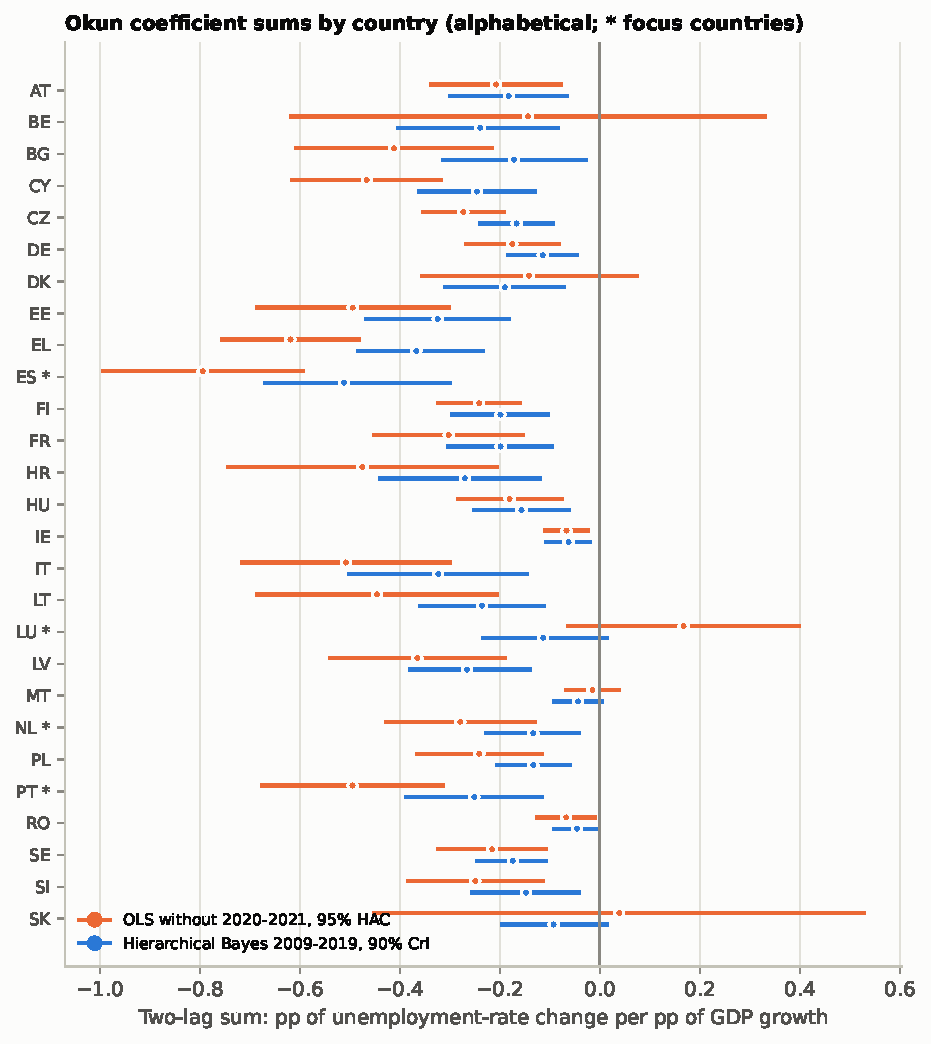
\includegraphics[width=0.78\textwidth]{fig1_countries.pdf}
\caption{Two-lag sums by country. Orange: OLS without 2020--2021 with 95\% HAC intervals.
Blue: hierarchical Bayesian posterior median, 2009--2019, with 90\% credible intervals.
Alphabetical order; focus countries marked. The Bayesian estimand excludes the common
European factor, so the two are not expected to coincide.}\label{fig:countries}
\end{figure}
